% !TEX TS-program = pdflatex
% !TEX encoding = UTF-8 Unicode
\documentclass[border=0mm]{standalone}
% packages
\usepackage{tikz}
\usetikzlibrary{patterns}
\usepackage{amsmath,amssymb}
\usepackage{bm}
\usepackage{pgfplots}
\pgfplotsset{compat=1.15}
% start document
\begin{document}
% generated by ROOT (CERN)
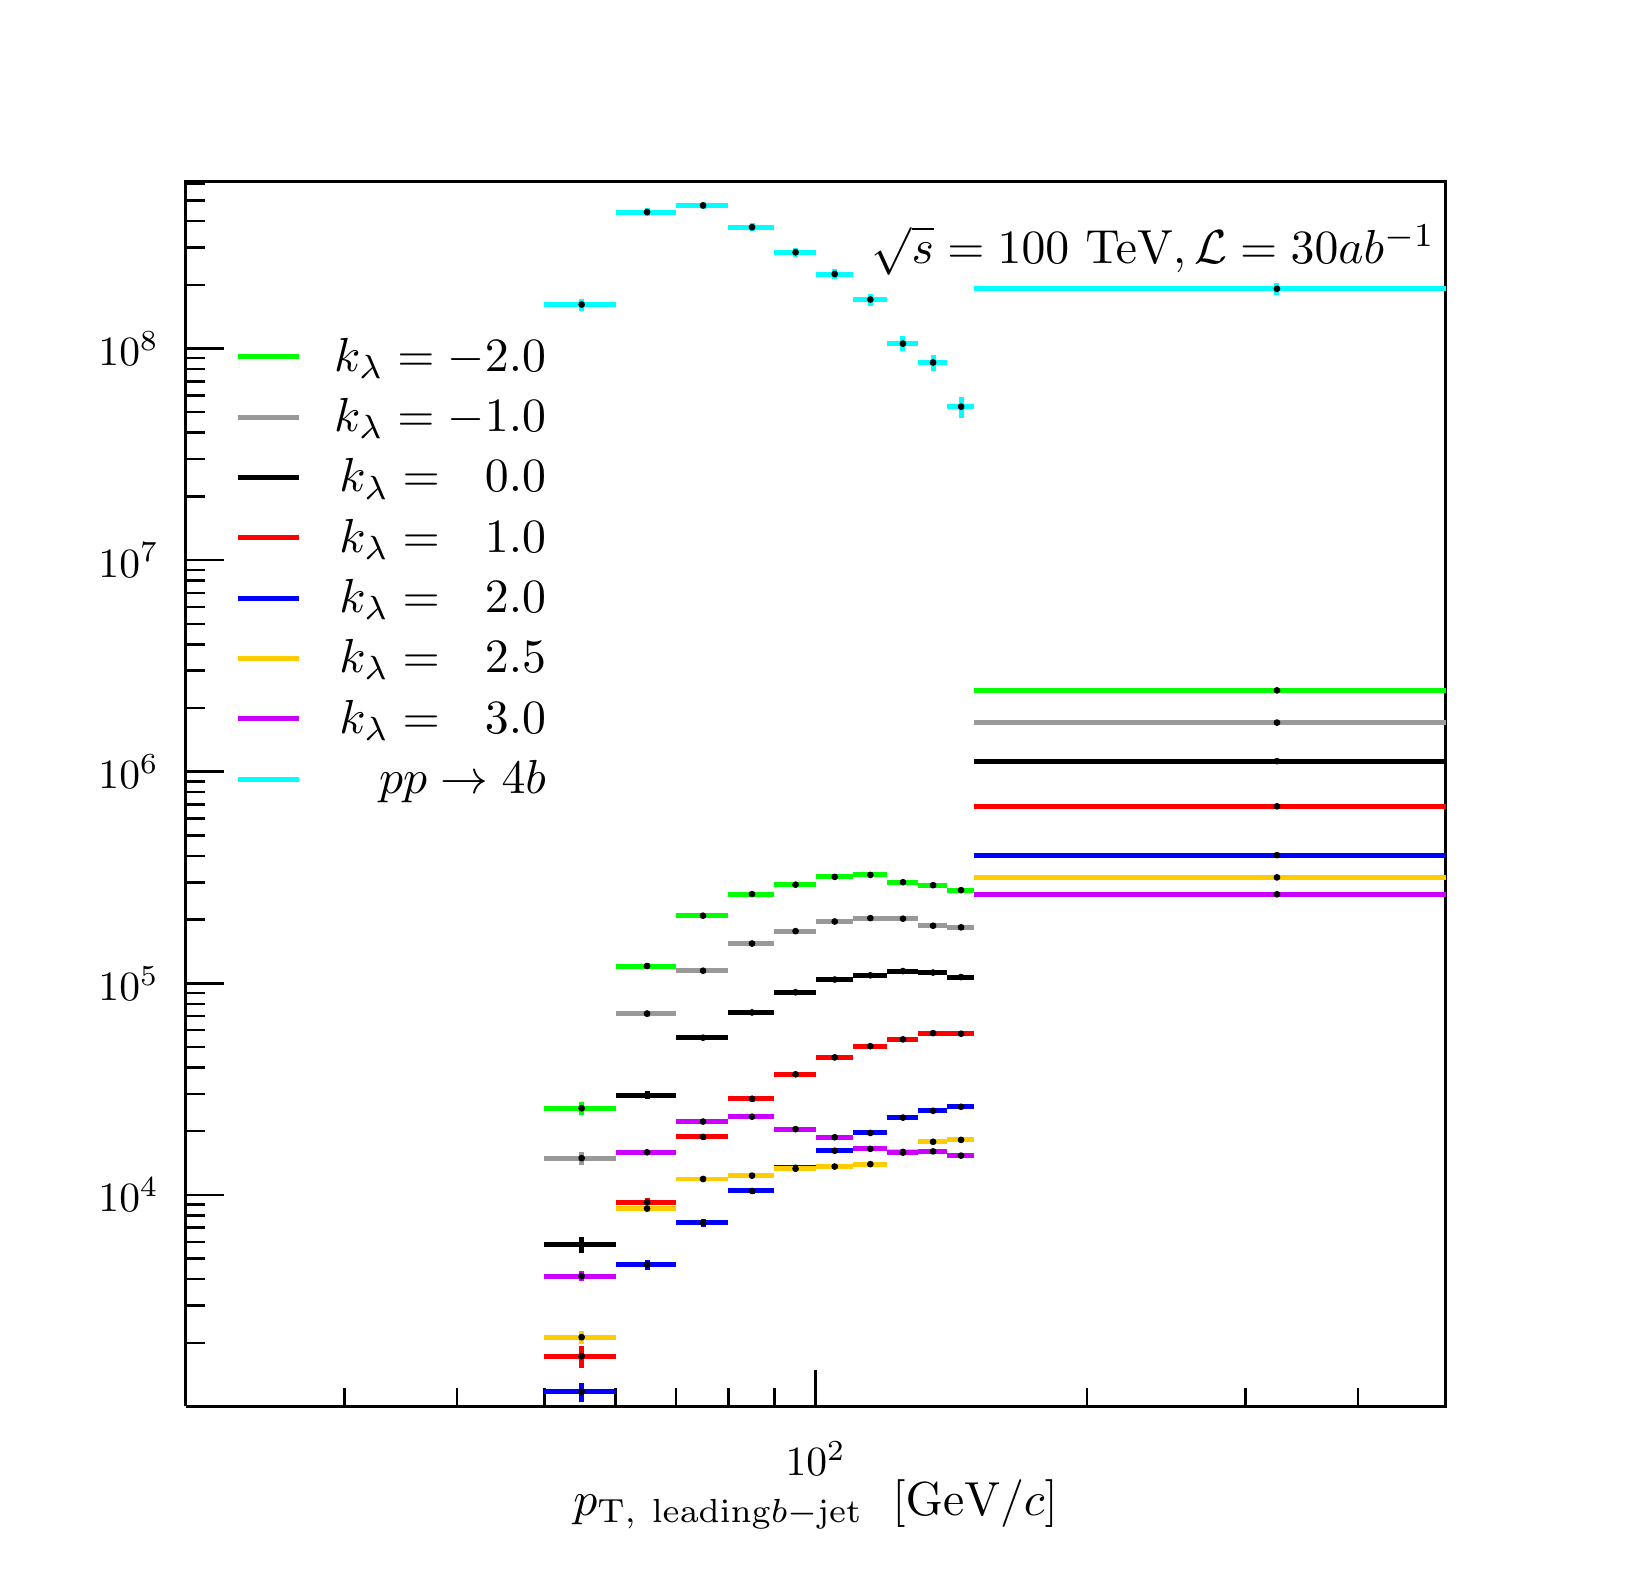
\begin{tikzpicture}
\pgfdeclareplotmark{cross} {
\pgfpathmoveto{\pgfpoint{-0.3\pgfplotmarksize}{\pgfplotmarksize}}
\pgfpathlineto{\pgfpoint{+0.3\pgfplotmarksize}{\pgfplotmarksize}}
\pgfpathlineto{\pgfpoint{+0.3\pgfplotmarksize}{0.3\pgfplotmarksize}}
\pgfpathlineto{\pgfpoint{+1\pgfplotmarksize}{0.3\pgfplotmarksize}}
\pgfpathlineto{\pgfpoint{+1\pgfplotmarksize}{-0.3\pgfplotmarksize}}
\pgfpathlineto{\pgfpoint{+0.3\pgfplotmarksize}{-0.3\pgfplotmarksize}}
\pgfpathlineto{\pgfpoint{+0.3\pgfplotmarksize}{-1.\pgfplotmarksize}}
\pgfpathlineto{\pgfpoint{-0.3\pgfplotmarksize}{-1.\pgfplotmarksize}}
\pgfpathlineto{\pgfpoint{-0.3\pgfplotmarksize}{-0.3\pgfplotmarksize}}
\pgfpathlineto{\pgfpoint{-1.\pgfplotmarksize}{-0.3\pgfplotmarksize}}
\pgfpathlineto{\pgfpoint{-1.\pgfplotmarksize}{0.3\pgfplotmarksize}}
\pgfpathlineto{\pgfpoint{-0.3\pgfplotmarksize}{0.3\pgfplotmarksize}}
\pgfpathclose
\pgfusepathqstroke
}
\pgfdeclareplotmark{cross*} {
\pgfpathmoveto{\pgfpoint{-0.3\pgfplotmarksize}{\pgfplotmarksize}}
\pgfpathlineto{\pgfpoint{+0.3\pgfplotmarksize}{\pgfplotmarksize}}
\pgfpathlineto{\pgfpoint{+0.3\pgfplotmarksize}{0.3\pgfplotmarksize}}
\pgfpathlineto{\pgfpoint{+1\pgfplotmarksize}{0.3\pgfplotmarksize}}
\pgfpathlineto{\pgfpoint{+1\pgfplotmarksize}{-0.3\pgfplotmarksize}}
\pgfpathlineto{\pgfpoint{+0.3\pgfplotmarksize}{-0.3\pgfplotmarksize}}
\pgfpathlineto{\pgfpoint{+0.3\pgfplotmarksize}{-1.\pgfplotmarksize}}
\pgfpathlineto{\pgfpoint{-0.3\pgfplotmarksize}{-1.\pgfplotmarksize}}
\pgfpathlineto{\pgfpoint{-0.3\pgfplotmarksize}{-0.3\pgfplotmarksize}}
\pgfpathlineto{\pgfpoint{-1.\pgfplotmarksize}{-0.3\pgfplotmarksize}}
\pgfpathlineto{\pgfpoint{-1.\pgfplotmarksize}{0.3\pgfplotmarksize}}
\pgfpathlineto{\pgfpoint{-0.3\pgfplotmarksize}{0.3\pgfplotmarksize}}
\pgfpathclose
\pgfusepathqfillstroke
}
\pgfdeclareplotmark{newstar} {
\pgfpathmoveto{\pgfqpoint{0pt}{\pgfplotmarksize}}
\pgfpathlineto{\pgfqpointpolar{44}{0.5\pgfplotmarksize}}
\pgfpathlineto{\pgfqpointpolar{18}{\pgfplotmarksize}}
\pgfpathlineto{\pgfqpointpolar{-20}{0.5\pgfplotmarksize}}
\pgfpathlineto{\pgfqpointpolar{-54}{\pgfplotmarksize}}
\pgfpathlineto{\pgfqpointpolar{-90}{0.5\pgfplotmarksize}}
\pgfpathlineto{\pgfqpointpolar{234}{\pgfplotmarksize}}
\pgfpathlineto{\pgfqpointpolar{198}{0.5\pgfplotmarksize}}
\pgfpathlineto{\pgfqpointpolar{162}{\pgfplotmarksize}}
\pgfpathlineto{\pgfqpointpolar{134}{0.5\pgfplotmarksize}}
\pgfpathclose
\pgfusepathqstroke
}
\pgfdeclareplotmark{newstar*} {
\pgfpathmoveto{\pgfqpoint{0pt}{\pgfplotmarksize}}
\pgfpathlineto{\pgfqpointpolar{44}{0.5\pgfplotmarksize}}
\pgfpathlineto{\pgfqpointpolar{18}{\pgfplotmarksize}}
\pgfpathlineto{\pgfqpointpolar{-20}{0.5\pgfplotmarksize}}
\pgfpathlineto{\pgfqpointpolar{-54}{\pgfplotmarksize}}
\pgfpathlineto{\pgfqpointpolar{-90}{0.5\pgfplotmarksize}}
\pgfpathlineto{\pgfqpointpolar{234}{\pgfplotmarksize}}
\pgfpathlineto{\pgfqpointpolar{198}{0.5\pgfplotmarksize}}
\pgfpathlineto{\pgfqpointpolar{162}{\pgfplotmarksize}}
\pgfpathlineto{\pgfqpointpolar{134}{0.5\pgfplotmarksize}}
\pgfpathclose
\pgfusepathqfillstroke
}
\definecolor{c}{rgb}{1,1,1};
\draw [color=c, fill=c] (0,0) rectangle (20,19.4486);
\draw [color=c, fill=c] (0,0) rectangle (20,19.4486);
\draw [color=c, fill=c] (2,1.94486) rectangle (18,17.5038);
\definecolor{c}{rgb}{0,0,0};
\draw [c,line width=0.9] (2,1.94486) -- (2,17.5038) -- (18,17.5038) -- (18,1.94486) -- (2,1.94486);
\definecolor{c}{rgb}{1,1,1};
\draw [color=c, fill=c] (2,1.94486) rectangle (18,17.5038);
\definecolor{c}{rgb}{0,0,0};
\draw [c,line width=0.9] (2,1.94486) -- (2,17.5038) -- (18,17.5038) -- (18,1.94486) -- (2,1.94486);
\definecolor{c}{rgb}{0,1,1};
\draw [c,line width=1.8] (7.02834,15.8598) -- (7.02834,15.9393);
\draw [c,line width=1.8] (7.02834,15.9393) -- (7.02834,16.0136);
\draw [c,line width=1.8] (6.55459,15.9393) -- (7.02834,15.9393);
\draw [c,line width=1.8] (7.02834,15.9393) -- (7.46085,15.9393);
\definecolor{c}{rgb}{0,0,0};
\foreach \P in {(7.02834,15.9393)}{\draw[mark options={color=c,fill=c},mark size=2.402402pt,mark=*,mark size=1pt] plot coordinates {\P};}
\definecolor{c}{rgb}{0,1,1};
\draw [c,line width=1.8] (7.85872,17.0665) -- (7.85872,17.1139);
\draw [c,line width=1.8] (7.85872,17.1139) -- (7.85872,17.1594);
\draw [c,line width=1.8] (7.46085,17.1139) -- (7.85872,17.1139);
\draw [c,line width=1.8] (7.85872,17.1139) -- (8.22708,17.1139);
\definecolor{c}{rgb}{0,0,0};
\foreach \P in {(7.85872,17.1139)}{\draw[mark options={color=c,fill=c},mark size=2.402402pt,mark=*,mark size=1pt] plot coordinates {\P};}
\definecolor{c}{rgb}{0,1,1};
\draw [c,line width=1.8] (8.57002,17.1519) -- (8.57002,17.1976);
\draw [c,line width=1.8] (8.57002,17.1976) -- (8.57002,17.2415);
\draw [c,line width=1.8] (8.22708,17.1976) -- (8.57002,17.1976);
\draw [c,line width=1.8] (8.57002,17.1976) -- (8.89083,17.1976);
\definecolor{c}{rgb}{0,0,0};
\foreach \P in {(8.57002,17.1976)}{\draw[mark options={color=c,fill=c},mark size=2.402402pt,mark=*,mark size=1pt] plot coordinates {\P};}
\definecolor{c}{rgb}{0,1,1};
\draw [c,line width=1.8] (9.19217,16.87) -- (9.19217,16.9216);
\draw [c,line width=1.8] (9.19217,16.9216) -- (9.19217,16.9709);
\draw [c,line width=1.8] (8.89083,16.9216) -- (9.19217,16.9216);
\draw [c,line width=1.8] (9.19217,16.9216) -- (9.47629,16.9216);
\definecolor{c}{rgb}{0,0,0};
\foreach \P in {(9.19217,16.9216)}{\draw[mark options={color=c,fill=c},mark size=2.402402pt,mark=*,mark size=1pt] plot coordinates {\P};}
\definecolor{c}{rgb}{0,1,1};
\draw [c,line width=1.8] (9.74504,16.5439) -- (9.74504,16.6031);
\draw [c,line width=1.8] (9.74504,16.6031) -- (9.74504,16.6595);
\draw [c,line width=1.8] (9.47629,16.6031) -- (9.74504,16.6031);
\draw [c,line width=1.8] (9.74504,16.6031) -- (10,16.6031);
\definecolor{c}{rgb}{0,0,0};
\foreach \P in {(9.74504,16.6031)}{\draw[mark options={color=c,fill=c},mark size=2.402402pt,mark=*,mark size=1pt] plot coordinates {\P};}
\definecolor{c}{rgb}{0,1,1};
\draw [c,line width=1.8] (10.2425,16.26) -- (10.2425,16.3269);
\draw [c,line width=1.8] (10.2425,16.3269) -- (10.2425,16.3902);
\draw [c,line width=1.8] (10,16.3269) -- (10.2425,16.3269);
\draw [c,line width=1.8] (10.2425,16.3269) -- (10.4738,16.3269);
\definecolor{c}{rgb}{0,0,0};
\foreach \P in {(10.2425,16.3269)}{\draw[mark options={color=c,fill=c},mark size=2.402402pt,mark=*,mark size=1pt] plot coordinates {\P};}
\definecolor{c}{rgb}{0,1,1};
\draw [c,line width=1.8] (10.6947,15.9259) -- (10.6947,16.0032);
\draw [c,line width=1.8] (10.6947,16.0032) -- (10.6947,16.0756);
\draw [c,line width=1.8] (10.4738,16.0032) -- (10.6947,16.0032);
\draw [c,line width=1.8] (10.6947,16.0032) -- (10.9063,16.0032);
\definecolor{c}{rgb}{0,0,0};
\foreach \P in {(10.6947,16.0032)}{\draw[mark options={color=c,fill=c},mark size=2.402402pt,mark=*,mark size=1pt] plot coordinates {\P};}
\definecolor{c}{rgb}{0,1,1};
\draw [c,line width=1.8] (11.1092,15.344) -- (11.1092,15.4431);
\draw [c,line width=1.8] (11.1092,15.4431) -- (11.1092,15.5344);
\draw [c,line width=1.8] (10.9063,15.4431) -- (11.1092,15.4431);
\draw [c,line width=1.8] (11.1092,15.4431) -- (11.3041,15.4431);
\definecolor{c}{rgb}{0,0,0};
\foreach \P in {(11.1092,15.4431)}{\draw[mark options={color=c,fill=c},mark size=2.402402pt,mark=*,mark size=1pt] plot coordinates {\P};}
\definecolor{c}{rgb}{0,1,1};
\draw [c,line width=1.8] (11.4917,15.0935) -- (11.4917,15.2038);
\draw [c,line width=1.8] (11.4917,15.2038) -- (11.4917,15.3045);
\draw [c,line width=1.8] (11.3041,15.2038) -- (11.4917,15.2038);
\draw [c,line width=1.8] (11.4917,15.2038) -- (11.6725,15.2038);
\definecolor{c}{rgb}{0,0,0};
\foreach \P in {(11.4917,15.2038)}{\draw[mark options={color=c,fill=c},mark size=2.402402pt,mark=*,mark size=1pt] plot coordinates {\P};}
\definecolor{c}{rgb}{0,1,1};
\draw [c,line width=1.8] (11.8469,14.4997) -- (11.8469,14.6419);
\draw [c,line width=1.8] (11.8469,14.6419) -- (11.8469,14.7686);
\draw [c,line width=1.8] (11.6725,14.6419) -- (11.8469,14.6419);
\draw [c,line width=1.8] (11.8469,14.6419) -- (12.0154,14.6419);
\definecolor{c}{rgb}{0,0,0};
\foreach \P in {(11.8469,14.6419)}{\draw[mark options={color=c,fill=c},mark size=2.402402pt,mark=*,mark size=1pt] plot coordinates {\P};}
\definecolor{c}{rgb}{0,1,1};
\draw [c,line width=1.8] (15.8587,16.0658) -- (15.8587,16.1385);
\draw [c,line width=1.8] (15.8587,16.1385) -- (15.8587,16.2069);
\draw [c,line width=1.8] (12.0154,16.1385) -- (15.8587,16.1385);
\draw [c,line width=1.8] (15.8587,16.1385) -- (18,16.1385);
\definecolor{c}{rgb}{0,0,0};
\foreach \P in {(15.8587,16.1385)}{\draw[mark options={color=c,fill=c},mark size=2.402402pt,mark=*,mark size=1pt] plot coordinates {\P};}
\draw [c,line width=0.9] (2,1.94486) -- (18,1.94486);
\draw [c,line width=0.9] (4.01543,2.17825) -- (4.01543,1.94486);
\draw [c,line width=0.9] (5.4454,2.17825) -- (5.4454,1.94486);
\draw [c,line width=0.9] (6.55458,2.17825) -- (6.55458,1.94486);
\draw [c,line width=0.9] (7.46084,2.17825) -- (7.46084,1.94486);
\draw [c,line width=0.9] (8.22708,2.17825) -- (8.22708,1.94486);
\draw [c,line width=0.9] (8.89082,2.17825) -- (8.89082,1.94486);
\draw [c,line width=0.9] (9.47628,2.17825) -- (9.47628,1.94486);
\draw [c,line width=0.9] (9.99999,2.41163) -- (9.99999,1.94486);
\draw [anchor=base] (9.99999,1.06481) node[scale=1.50291, color=c, rotate=0]{$10^{2}$};
\draw [c,line width=0.9] (13.4454,2.17825) -- (13.4454,1.94486);
\draw [c,line width=0.9] (15.4608,2.17825) -- (15.4608,1.94486);
\draw [c,line width=0.9] (16.8908,2.17825) -- (16.8908,1.94486);
\draw [c,line width=0.9] (18,2.17825) -- (18,1.94486);
\draw (10,0.700151) node[scale=1.72557, color=c, rotate=0]{$ p_{\text{T}, ~\text{leading} b-\text{jet~}} ~[\text{GeV}/c]$};
\draw [c,line width=0.9] (2,1.94486) -- (2,17.5038);
\draw [c,line width=0.9] (2.24,2.75379) -- (2,2.75379);
\draw [c,line width=0.9] (2.24,3.22699) -- (2,3.22699);
\draw [c,line width=0.9] (2.24,3.56272) -- (2,3.56272);
\draw [c,line width=0.9] (2.24,3.82314) -- (2,3.82314);
\draw [c,line width=0.9] (2.24,4.03592) -- (2,4.03592);
\draw [c,line width=0.9] (2.24,4.21582) -- (2,4.21582);
\draw [c,line width=0.9] (2.24,4.37166) -- (2,4.37166);
\draw [c,line width=0.9] (2.24,4.50911) -- (2,4.50911);
\draw [c,line width=0.9] (2.48,4.63207) -- (2,4.63207);
\draw [anchor= east] (1.844,4.63207) node[scale=1.50291, color=c, rotate=0]{$10^{4}$};
\draw [c,line width=0.9] (2.24,5.44101) -- (2,5.44101);
\draw [c,line width=0.9] (2.24,5.9142) -- (2,5.9142);
\draw [c,line width=0.9] (2.24,6.24994) -- (2,6.24994);
\draw [c,line width=0.9] (2.24,6.51036) -- (2,6.51036);
\draw [c,line width=0.9] (2.24,6.72313) -- (2,6.72313);
\draw [c,line width=0.9] (2.24,6.90303) -- (2,6.90303);
\draw [c,line width=0.9] (2.24,7.05887) -- (2,7.05887);
\draw [c,line width=0.9] (2.24,7.19633) -- (2,7.19633);
\draw [c,line width=0.9] (2.48,7.31929) -- (2,7.31929);
\draw [anchor= east] (1.844,7.31929) node[scale=1.50291, color=c, rotate=0]{$10^{5}$};
\draw [c,line width=0.9] (2.24,8.12822) -- (2,8.12822);
\draw [c,line width=0.9] (2.24,8.60142) -- (2,8.60142);
\draw [c,line width=0.9] (2.24,8.93715) -- (2,8.93715);
\draw [c,line width=0.9] (2.24,9.19757) -- (2,9.19757);
\draw [c,line width=0.9] (2.24,9.41035) -- (2,9.41035);
\draw [c,line width=0.9] (2.24,9.59025) -- (2,9.59025);
\draw [c,line width=0.9] (2.24,9.74609) -- (2,9.74609);
\draw [c,line width=0.9] (2.24,9.88354) -- (2,9.88354);
\draw [c,line width=0.9] (2.48,10.0065) -- (2,10.0065);
\draw [anchor= east] (1.844,10.0065) node[scale=1.50291, color=c, rotate=0]{$10^{6}$};
\draw [c,line width=0.9] (2.24,10.8154) -- (2,10.8154);
\draw [c,line width=0.9] (2.24,11.2886) -- (2,11.2886);
\draw [c,line width=0.9] (2.24,11.6244) -- (2,11.6244);
\draw [c,line width=0.9] (2.24,11.8848) -- (2,11.8848);
\draw [c,line width=0.9] (2.24,12.0976) -- (2,12.0976);
\draw [c,line width=0.9] (2.24,12.2775) -- (2,12.2775);
\draw [c,line width=0.9] (2.24,12.4333) -- (2,12.4333);
\draw [c,line width=0.9] (2.24,12.5708) -- (2,12.5708);
\draw [c,line width=0.9] (2.48,12.6937) -- (2,12.6937);
\draw [anchor= east] (1.844,12.6937) node[scale=1.50291, color=c, rotate=0]{$10^{7}$};
\draw [c,line width=0.9] (2.24,13.5026) -- (2,13.5026);
\draw [c,line width=0.9] (2.24,13.9758) -- (2,13.9758);
\draw [c,line width=0.9] (2.24,14.3116) -- (2,14.3116);
\draw [c,line width=0.9] (2.24,14.572) -- (2,14.572);
\draw [c,line width=0.9] (2.24,14.7848) -- (2,14.7848);
\draw [c,line width=0.9] (2.24,14.9647) -- (2,14.9647);
\draw [c,line width=0.9] (2.24,15.1205) -- (2,15.1205);
\draw [c,line width=0.9] (2.24,15.258) -- (2,15.258);
\draw [c,line width=0.9] (2.48,15.3809) -- (2,15.3809);
\draw [anchor= east] (1.844,15.3809) node[scale=1.50291, color=c, rotate=0]{$10^{8}$};
\draw [c,line width=0.9] (2.24,16.1899) -- (2,16.1899);
\draw [c,line width=0.9] (2.24,16.6631) -- (2,16.6631);
\draw [c,line width=0.9] (2.24,16.9988) -- (2,16.9988);
\draw [c,line width=0.9] (2.24,17.2592) -- (2,17.2592);
\draw [c,line width=0.9] (2.24,17.472) -- (2,17.472);
\definecolor{c}{rgb}{0,1,0};
\draw [c,line width=1.8] (7.02834,5.64775) -- (7.02834,5.73203);
\draw [c,line width=1.8] (7.02834,5.73203) -- (7.02834,5.81063);
\draw [c,line width=1.8] (6.55459,5.73203) -- (7.02834,5.73203);
\draw [c,line width=1.8] (7.02834,5.73203) -- (7.46085,5.73203);
\definecolor{c}{rgb}{0,0,0};
\foreach \P in {(7.02834,5.73203)}{\draw[mark options={color=c,fill=c},mark size=2.402402pt,mark=*,mark size=1pt] plot coordinates {\P};}
\definecolor{c}{rgb}{0,1,0};
\draw [c,line width=1.8] (7.85872,7.49973) -- (7.85872,7.53786);
\draw [c,line width=1.8] (7.85872,7.53786) -- (7.85872,7.57478);
\draw [c,line width=1.8] (7.46085,7.53786) -- (7.85872,7.53786);
\draw [c,line width=1.8] (7.85872,7.53786) -- (8.22708,7.53786);
\definecolor{c}{rgb}{0,0,0};
\foreach \P in {(7.85872,7.53786)}{\draw[mark options={color=c,fill=c},mark size=2.402402pt,mark=*,mark size=1pt] plot coordinates {\P};}
\definecolor{c}{rgb}{0,1,0};
\draw [c,line width=1.8] (8.57002,8.14822) -- (8.57002,8.17709);
\draw [c,line width=1.8] (8.57002,8.17709) -- (8.57002,8.20527);
\draw [c,line width=1.8] (8.22708,8.17709) -- (8.57002,8.17709);
\draw [c,line width=1.8] (8.57002,8.17709) -- (8.89083,8.17709);
\definecolor{c}{rgb}{0,0,0};
\foreach \P in {(8.57002,8.17709)}{\draw[mark options={color=c,fill=c},mark size=2.402402pt,mark=*,mark size=1pt] plot coordinates {\P};}
\definecolor{c}{rgb}{0,1,0};
\draw [c,line width=1.8] (9.19217,8.42601) -- (9.19217,8.45165);
\draw [c,line width=1.8] (9.19217,8.45165) -- (9.19217,8.47674);
\draw [c,line width=1.8] (8.89083,8.45165) -- (9.19217,8.45165);
\draw [c,line width=1.8] (9.19217,8.45165) -- (9.47629,8.45165);
\definecolor{c}{rgb}{0,0,0};
\foreach \P in {(9.19217,8.45165)}{\draw[mark options={color=c,fill=c},mark size=2.402402pt,mark=*,mark size=1pt] plot coordinates {\P};}
\definecolor{c}{rgb}{0,1,0};
\draw [c,line width=1.8] (9.74504,8.54712) -- (9.74504,8.57146);
\draw [c,line width=1.8] (9.74504,8.57146) -- (9.74504,8.59531);
\draw [c,line width=1.8] (9.47629,8.57146) -- (9.74504,8.57146);
\draw [c,line width=1.8] (9.74504,8.57146) -- (10,8.57146);
\definecolor{c}{rgb}{0,0,0};
\foreach \P in {(9.74504,8.57146)}{\draw[mark options={color=c,fill=c},mark size=2.402402pt,mark=*,mark size=1pt] plot coordinates {\P};}
\definecolor{c}{rgb}{0,1,0};
\draw [c,line width=1.8] (10.2425,8.64724) -- (10.2425,8.67056);
\draw [c,line width=1.8] (10.2425,8.67056) -- (10.2425,8.69342);
\draw [c,line width=1.8] (10,8.67056) -- (10.2425,8.67056);
\draw [c,line width=1.8] (10.2425,8.67056) -- (10.4738,8.67056);
\definecolor{c}{rgb}{0,0,0};
\foreach \P in {(10.2425,8.67056)}{\draw[mark options={color=c,fill=c},mark size=2.402402pt,mark=*,mark size=1pt] plot coordinates {\P};}
\definecolor{c}{rgb}{0,1,0};
\draw [c,line width=1.8] (10.6947,8.67235) -- (10.6947,8.69542);
\draw [c,line width=1.8] (10.6947,8.69542) -- (10.6947,8.71804);
\draw [c,line width=1.8] (10.4738,8.69542) -- (10.6947,8.69542);
\draw [c,line width=1.8] (10.6947,8.69542) -- (10.9063,8.69542);
\definecolor{c}{rgb}{0,0,0};
\foreach \P in {(10.6947,8.69542)}{\draw[mark options={color=c,fill=c},mark size=2.402402pt,mark=*,mark size=1pt] plot coordinates {\P};}
\definecolor{c}{rgb}{0,1,0};
\draw [c,line width=1.8] (11.1092,8.57885) -- (11.1092,8.60286);
\draw [c,line width=1.8] (11.1092,8.60286) -- (11.1092,8.62639);
\draw [c,line width=1.8] (10.9063,8.60286) -- (11.1092,8.60286);
\draw [c,line width=1.8] (11.1092,8.60286) -- (11.3041,8.60286);
\definecolor{c}{rgb}{0,0,0};
\foreach \P in {(11.1092,8.60286)}{\draw[mark options={color=c,fill=c},mark size=2.402402pt,mark=*,mark size=1pt] plot coordinates {\P};}
\definecolor{c}{rgb}{0,1,0};
\draw [c,line width=1.8] (11.4917,8.54057) -- (11.4917,8.56498);
\draw [c,line width=1.8] (11.4917,8.56498) -- (11.4917,8.58889);
\draw [c,line width=1.8] (11.3041,8.56498) -- (11.4917,8.56498);
\draw [c,line width=1.8] (11.4917,8.56498) -- (11.6725,8.56498);
\definecolor{c}{rgb}{0,0,0};
\foreach \P in {(11.4917,8.56498)}{\draw[mark options={color=c,fill=c},mark size=2.402402pt,mark=*,mark size=1pt] plot coordinates {\P};}
\definecolor{c}{rgb}{0,1,0};
\draw [c,line width=1.8] (11.8469,8.47671) -- (11.8469,8.5018);
\draw [c,line width=1.8] (11.8469,8.5018) -- (11.8469,8.52636);
\draw [c,line width=1.8] (11.6725,8.5018) -- (11.8469,8.5018);
\draw [c,line width=1.8] (11.8469,8.5018) -- (12.0154,8.5018);
\definecolor{c}{rgb}{0,0,0};
\foreach \P in {(11.8469,8.5018)}{\draw[mark options={color=c,fill=c},mark size=2.402402pt,mark=*,mark size=1pt] plot coordinates {\P};}
\definecolor{c}{rgb}{0,1,0};
\draw [c,line width=1.8] (15.8587,11.0305) -- (15.8587,11.0389);
\draw [c,line width=1.8] (15.8587,11.0389) -- (15.8587,11.0473);
\draw [c,line width=1.8] (12.0154,11.0389) -- (15.8587,11.0389);
\draw [c,line width=1.8] (15.8587,11.0389) -- (18,11.0389);
\definecolor{c}{rgb}{0,0,0};
\foreach \P in {(15.8587,11.0389)}{\draw[mark options={color=c,fill=c},mark size=2.402402pt,mark=*,mark size=1pt] plot coordinates {\P};}
\definecolor{c}{rgb}{0.6,0.6,0.6};
\draw [c,line width=1.8] (7.02834,5.00979) -- (7.02834,5.09891);
\draw [c,line width=1.8] (7.02834,5.09891) -- (7.02834,5.1817);
\draw [c,line width=1.8] (6.55459,5.09891) -- (7.02834,5.09891);
\draw [c,line width=1.8] (7.02834,5.09891) -- (7.46085,5.09891);
\definecolor{c}{rgb}{0,0,0};
\foreach \P in {(7.02834,5.09891)}{\draw[mark options={color=c,fill=c},mark size=2.402402pt,mark=*,mark size=1pt] plot coordinates {\P};}
\definecolor{c}{rgb}{0.6,0.6,0.6};
\draw [c,line width=1.8] (7.85872,6.89505) -- (7.85872,6.9348);
\draw [c,line width=1.8] (7.85872,6.9348) -- (7.85872,6.97323);
\draw [c,line width=1.8] (7.46085,6.9348) -- (7.85872,6.9348);
\draw [c,line width=1.8] (7.85872,6.9348) -- (8.22708,6.9348);
\definecolor{c}{rgb}{0,0,0};
\foreach \P in {(7.85872,6.9348)}{\draw[mark options={color=c,fill=c},mark size=2.402402pt,mark=*,mark size=1pt] plot coordinates {\P};}
\definecolor{c}{rgb}{0.6,0.6,0.6};
\draw [c,line width=1.8] (8.57002,7.44768) -- (8.57002,7.47905);
\draw [c,line width=1.8] (8.57002,7.47905) -- (8.57002,7.5096);
\draw [c,line width=1.8] (8.22708,7.47905) -- (8.57002,7.47905);
\draw [c,line width=1.8] (8.57002,7.47905) -- (8.89083,7.47905);
\definecolor{c}{rgb}{0,0,0};
\foreach \P in {(8.57002,7.47905)}{\draw[mark options={color=c,fill=c},mark size=2.402402pt,mark=*,mark size=1pt] plot coordinates {\P};}
\definecolor{c}{rgb}{0.6,0.6,0.6};
\draw [c,line width=1.8] (9.19217,7.79698) -- (9.19217,7.82398);
\draw [c,line width=1.8] (9.19217,7.82398) -- (9.19217,7.85038);
\draw [c,line width=1.8] (8.89083,7.82398) -- (9.19217,7.82398);
\draw [c,line width=1.8] (9.19217,7.82398) -- (9.47629,7.82398);
\definecolor{c}{rgb}{0,0,0};
\foreach \P in {(9.19217,7.82398)}{\draw[mark options={color=c,fill=c},mark size=2.402402pt,mark=*,mark size=1pt] plot coordinates {\P};}
\definecolor{c}{rgb}{0.6,0.6,0.6};
\draw [c,line width=1.8] (9.74504,7.9562) -- (9.74504,7.98142);
\draw [c,line width=1.8] (9.74504,7.98142) -- (9.74504,8.00611);
\draw [c,line width=1.8] (9.47629,7.98142) -- (9.74504,7.98142);
\draw [c,line width=1.8] (9.74504,7.98142) -- (10,7.98142);
\definecolor{c}{rgb}{0,0,0};
\foreach \P in {(9.74504,7.98142)}{\draw[mark options={color=c,fill=c},mark size=2.402402pt,mark=*,mark size=1pt] plot coordinates {\P};}
\definecolor{c}{rgb}{0.6,0.6,0.6};
\draw [c,line width=1.8] (10.2425,8.07998) -- (10.2425,8.1039);
\draw [c,line width=1.8] (10.2425,8.1039) -- (10.2425,8.12735);
\draw [c,line width=1.8] (10,8.1039) -- (10.2425,8.1039);
\draw [c,line width=1.8] (10.2425,8.1039) -- (10.4738,8.1039);
\definecolor{c}{rgb}{0,0,0};
\foreach \P in {(10.2425,8.1039)}{\draw[mark options={color=c,fill=c},mark size=2.402402pt,mark=*,mark size=1pt] plot coordinates {\P};}
\definecolor{c}{rgb}{0.6,0.6,0.6};
\draw [c,line width=1.8] (10.6947,8.12334) -- (10.6947,8.14683);
\draw [c,line width=1.8] (10.6947,8.14683) -- (10.6947,8.16984);
\draw [c,line width=1.8] (10.4738,8.14683) -- (10.6947,8.14683);
\draw [c,line width=1.8] (10.6947,8.14683) -- (10.9063,8.14683);
\definecolor{c}{rgb}{0,0,0};
\foreach \P in {(10.6947,8.14683)}{\draw[mark options={color=c,fill=c},mark size=2.402402pt,mark=*,mark size=1pt] plot coordinates {\P};}
\definecolor{c}{rgb}{0.6,0.6,0.6};
\draw [c,line width=1.8] (11.1092,8.11583) -- (11.1092,8.13939);
\draw [c,line width=1.8] (11.1092,8.13939) -- (11.1092,8.16248);
\draw [c,line width=1.8] (10.9063,8.13939) -- (11.1092,8.13939);
\draw [c,line width=1.8] (11.1092,8.13939) -- (11.3041,8.13939);
\definecolor{c}{rgb}{0,0,0};
\foreach \P in {(11.1092,8.13939)}{\draw[mark options={color=c,fill=c},mark size=2.402402pt,mark=*,mark size=1pt] plot coordinates {\P};}
\definecolor{c}{rgb}{0.6,0.6,0.6};
\draw [c,line width=1.8] (11.4917,8.02584) -- (11.4917,8.05032);
\draw [c,line width=1.8] (11.4917,8.05032) -- (11.4917,8.0743);
\draw [c,line width=1.8] (11.3041,8.05032) -- (11.4917,8.05032);
\draw [c,line width=1.8] (11.4917,8.05032) -- (11.6725,8.05032);
\definecolor{c}{rgb}{0,0,0};
\foreach \P in {(11.4917,8.05032)}{\draw[mark options={color=c,fill=c},mark size=2.402402pt,mark=*,mark size=1pt] plot coordinates {\P};}
\definecolor{c}{rgb}{0.6,0.6,0.6};
\draw [c,line width=1.8] (11.8469,8.00481) -- (11.8469,8.02951);
\draw [c,line width=1.8] (11.8469,8.02951) -- (11.8469,8.05371);
\draw [c,line width=1.8] (11.6725,8.02951) -- (11.8469,8.02951);
\draw [c,line width=1.8] (11.8469,8.02951) -- (12.0154,8.02951);
\definecolor{c}{rgb}{0,0,0};
\foreach \P in {(11.8469,8.02951)}{\draw[mark options={color=c,fill=c},mark size=2.402402pt,mark=*,mark size=1pt] plot coordinates {\P};}
\definecolor{c}{rgb}{0.6,0.6,0.6};
\draw [c,line width=1.8] (15.8587,10.6217) -- (15.8587,10.6298);
\draw [c,line width=1.8] (15.8587,10.6298) -- (15.8587,10.6378);
\draw [c,line width=1.8] (12.0154,10.6298) -- (15.8587,10.6298);
\draw [c,line width=1.8] (15.8587,10.6298) -- (18,10.6298);
\definecolor{c}{rgb}{0,0,0};
\foreach \P in {(15.8587,10.6298)}{\draw[mark options={color=c,fill=c},mark size=2.402402pt,mark=*,mark size=1pt] plot coordinates {\P};}
\draw [c,line width=1.8] (7.02834,3.89101) -- (7.02834,4.00129);
\draw [c,line width=1.8] (7.02834,4.00129) -- (7.02834,4.10204);
\draw [c,line width=1.8] (6.55459,4.00129) -- (7.02834,4.00129);
\draw [c,line width=1.8] (7.02834,4.00129) -- (7.46085,4.00129);
\foreach \P in {(7.02834,4.00129)}{\draw[mark options={color=c,fill=c},mark size=2.402402pt,mark=*,mark size=1pt] plot coordinates {\P};}
\draw [c,line width=1.8] (7.85872,5.85266) -- (7.85872,5.90026);
\draw [c,line width=1.8] (7.85872,5.90026) -- (7.85872,5.946);
\draw [c,line width=1.8] (7.46085,5.90026) -- (7.85872,5.90026);
\draw [c,line width=1.8] (7.85872,5.90026) -- (8.22708,5.90026);
\foreach \P in {(7.85872,5.90026)}{\draw[mark options={color=c,fill=c},mark size=2.402402pt,mark=*,mark size=1pt] plot coordinates {\P};}
\draw [c,line width=1.8] (8.57002,6.59349) -- (8.57002,6.62814);
\draw [c,line width=1.8] (8.57002,6.62814) -- (8.57002,6.6618);
\draw [c,line width=1.8] (8.22708,6.62814) -- (8.57002,6.62814);
\draw [c,line width=1.8] (8.57002,6.62814) -- (8.89083,6.62814);
\foreach \P in {(8.57002,6.62814)}{\draw[mark options={color=c,fill=c},mark size=2.402402pt,mark=*,mark size=1pt] plot coordinates {\P};}
\draw [c,line width=1.8] (9.19217,6.91839) -- (9.19217,6.94854);
\draw [c,line width=1.8] (9.19217,6.94854) -- (9.19217,6.97794);
\draw [c,line width=1.8] (8.89083,6.94854) -- (9.19217,6.94854);
\draw [c,line width=1.8] (9.19217,6.94854) -- (9.47629,6.94854);
\foreach \P in {(9.19217,6.94854)}{\draw[mark options={color=c,fill=c},mark size=2.402402pt,mark=*,mark size=1pt] plot coordinates {\P};}
\draw [c,line width=1.8] (9.74504,7.17818) -- (9.74504,7.20516);
\draw [c,line width=1.8] (9.74504,7.20516) -- (9.74504,7.23153);
\draw [c,line width=1.8] (9.47629,7.20516) -- (9.74504,7.20516);
\draw [c,line width=1.8] (9.74504,7.20516) -- (10,7.20516);
\foreach \P in {(9.74504,7.20516)}{\draw[mark options={color=c,fill=c},mark size=2.402402pt,mark=*,mark size=1pt] plot coordinates {\P};}
\draw [c,line width=1.8] (10.2425,7.34192) -- (10.2425,7.36707);
\draw [c,line width=1.8] (10.2425,7.36707) -- (10.2425,7.39169);
\draw [c,line width=1.8] (10,7.36707) -- (10.2425,7.36707);
\draw [c,line width=1.8] (10.2425,7.36707) -- (10.4738,7.36707);
\foreach \P in {(10.2425,7.36707)}{\draw[mark options={color=c,fill=c},mark size=2.402402pt,mark=*,mark size=1pt] plot coordinates {\P};}
\draw [c,line width=1.8] (10.6947,7.3959) -- (10.6947,7.42047);
\draw [c,line width=1.8] (10.6947,7.42047) -- (10.6947,7.44454);
\draw [c,line width=1.8] (10.4738,7.42047) -- (10.6947,7.42047);
\draw [c,line width=1.8] (10.6947,7.42047) -- (10.9063,7.42047);
\foreach \P in {(10.6947,7.42047)}{\draw[mark options={color=c,fill=c},mark size=2.402402pt,mark=*,mark size=1pt] plot coordinates {\P};}
\draw [c,line width=1.8] (11.1092,7.44994) -- (11.1092,7.47396);
\draw [c,line width=1.8] (11.1092,7.47396) -- (11.1092,7.49749);
\draw [c,line width=1.8] (10.9063,7.47396) -- (11.1092,7.47396);
\draw [c,line width=1.8] (11.1092,7.47396) -- (11.3041,7.47396);
\foreach \P in {(11.1092,7.47396)}{\draw[mark options={color=c,fill=c},mark size=2.402402pt,mark=*,mark size=1pt] plot coordinates {\P};}
\draw [c,line width=1.8] (11.4917,7.43121) -- (11.4917,7.45542);
\draw [c,line width=1.8] (11.4917,7.45542) -- (11.4917,7.47913);
\draw [c,line width=1.8] (11.3041,7.45542) -- (11.4917,7.45542);
\draw [c,line width=1.8] (11.4917,7.45542) -- (11.6725,7.45542);
\foreach \P in {(11.4917,7.45542)}{\draw[mark options={color=c,fill=c},mark size=2.402402pt,mark=*,mark size=1pt] plot coordinates {\P};}
\draw [c,line width=1.8] (11.8469,7.37367) -- (11.8469,7.39848);
\draw [c,line width=1.8] (11.8469,7.39848) -- (11.8469,7.42277);
\draw [c,line width=1.8] (11.6725,7.39848) -- (11.8469,7.39848);
\draw [c,line width=1.8] (11.8469,7.39848) -- (12.0154,7.39848);
\foreach \P in {(11.8469,7.39848)}{\draw[mark options={color=c,fill=c},mark size=2.402402pt,mark=*,mark size=1pt] plot coordinates {\P};}
\draw [c,line width=1.8] (15.8587,10.1331) -- (15.8587,10.1407);
\draw [c,line width=1.8] (15.8587,10.1407) -- (15.8587,10.1483);
\draw [c,line width=1.8] (12.0154,10.1407) -- (15.8587,10.1407);
\draw [c,line width=1.8] (15.8587,10.1407) -- (18,10.1407);
\foreach \P in {(15.8587,10.1407)}{\draw[mark options={color=c,fill=c},mark size=2.402402pt,mark=*,mark size=1pt] plot coordinates {\P};}
\definecolor{c}{rgb}{1,0,0};
\draw [c,line width=1.8] (7.02834,2.43556) -- (7.02834,2.58411);
\draw [c,line width=1.8] (7.02834,2.58411) -- (7.02834,2.71588);
\draw [c,line width=1.8] (6.55459,2.58411) -- (7.02834,2.58411);
\draw [c,line width=1.8] (7.02834,2.58411) -- (7.46085,2.58411);
\definecolor{c}{rgb}{0,0,0};
\foreach \P in {(7.02834,2.58411)}{\draw[mark options={color=c,fill=c},mark size=2.402402pt,mark=*,mark size=1pt] plot coordinates {\P};}
\definecolor{c}{rgb}{1,0,0};
\draw [c,line width=1.8] (7.85872,4.47463) -- (7.85872,4.53667);
\draw [c,line width=1.8] (7.85872,4.53667) -- (7.85872,4.59559);
\draw [c,line width=1.8] (7.46085,4.53667) -- (7.85872,4.53667);
\draw [c,line width=1.8] (7.85872,4.53667) -- (8.22708,4.53667);
\definecolor{c}{rgb}{0,0,0};
\foreach \P in {(7.85872,4.53667)}{\draw[mark options={color=c,fill=c},mark size=2.402402pt,mark=*,mark size=1pt] plot coordinates {\P};}
\definecolor{c}{rgb}{1,0,0};
\draw [c,line width=1.8] (8.57002,5.32575) -- (8.57002,5.36884);
\draw [c,line width=1.8] (8.57002,5.36884) -- (8.57002,5.4104);
\draw [c,line width=1.8] (8.22708,5.36884) -- (8.57002,5.36884);
\draw [c,line width=1.8] (8.57002,5.36884) -- (8.89083,5.36884);
\definecolor{c}{rgb}{0,0,0};
\foreach \P in {(8.57002,5.36884)}{\draw[mark options={color=c,fill=c},mark size=2.402402pt,mark=*,mark size=1pt] plot coordinates {\P};}
\definecolor{c}{rgb}{1,0,0};
\draw [c,line width=1.8] (9.19217,5.81782) -- (9.19217,5.85272);
\draw [c,line width=1.8] (9.19217,5.85272) -- (9.19217,5.88661);
\draw [c,line width=1.8] (8.89083,5.85272) -- (9.19217,5.85272);
\draw [c,line width=1.8] (9.19217,5.85272) -- (9.47629,5.85272);
\definecolor{c}{rgb}{0,0,0};
\foreach \P in {(9.19217,5.85272)}{\draw[mark options={color=c,fill=c},mark size=2.402402pt,mark=*,mark size=1pt] plot coordinates {\P};}
\definecolor{c}{rgb}{1,0,0};
\draw [c,line width=1.8] (9.74504,6.13261) -- (9.74504,6.16311);
\draw [c,line width=1.8] (9.74504,6.16311) -- (9.74504,6.19283);
\draw [c,line width=1.8] (9.47629,6.16311) -- (9.74504,6.16311);
\draw [c,line width=1.8] (9.74504,6.16311) -- (10,6.16311);
\definecolor{c}{rgb}{0,0,0};
\foreach \P in {(9.74504,6.16311)}{\draw[mark options={color=c,fill=c},mark size=2.402402pt,mark=*,mark size=1pt] plot coordinates {\P};}
\definecolor{c}{rgb}{1,0,0};
\draw [c,line width=1.8] (10.2425,6.3503) -- (10.2425,6.37809);
\draw [c,line width=1.8] (10.2425,6.37809) -- (10.2425,6.40522);
\draw [c,line width=1.8] (10,6.37809) -- (10.2425,6.37809);
\draw [c,line width=1.8] (10.2425,6.37809) -- (10.4738,6.37809);
\definecolor{c}{rgb}{0,0,0};
\foreach \P in {(10.2425,6.37809)}{\draw[mark options={color=c,fill=c},mark size=2.402402pt,mark=*,mark size=1pt] plot coordinates {\P};}
\definecolor{c}{rgb}{1,0,0};
\draw [c,line width=1.8] (10.6947,6.49408) -- (10.6947,6.5202);
\draw [c,line width=1.8] (10.6947,6.5202) -- (10.6947,6.54575);
\draw [c,line width=1.8] (10.4738,6.5202) -- (10.6947,6.5202);
\draw [c,line width=1.8] (10.6947,6.5202) -- (10.9063,6.5202);
\definecolor{c}{rgb}{0,0,0};
\foreach \P in {(10.6947,6.5202)}{\draw[mark options={color=c,fill=c},mark size=2.402402pt,mark=*,mark size=1pt] plot coordinates {\P};}
\definecolor{c}{rgb}{1,0,0};
\draw [c,line width=1.8] (11.1092,6.58206) -- (11.1092,6.60722);
\draw [c,line width=1.8] (11.1092,6.60722) -- (11.1092,6.63184);
\draw [c,line width=1.8] (10.9063,6.60722) -- (11.1092,6.60722);
\draw [c,line width=1.8] (11.1092,6.60722) -- (11.3041,6.60722);
\definecolor{c}{rgb}{0,0,0};
\foreach \P in {(11.1092,6.60722)}{\draw[mark options={color=c,fill=c},mark size=2.402402pt,mark=*,mark size=1pt] plot coordinates {\P};}
\definecolor{c}{rgb}{1,0,0};
\draw [c,line width=1.8] (11.4917,6.6619) -- (11.4917,6.68621);
\draw [c,line width=1.8] (11.4917,6.68621) -- (11.4917,6.71003);
\draw [c,line width=1.8] (11.3041,6.68621) -- (11.4917,6.68621);
\draw [c,line width=1.8] (11.4917,6.68621) -- (11.6725,6.68621);
\definecolor{c}{rgb}{0,0,0};
\foreach \P in {(11.4917,6.68621)}{\draw[mark options={color=c,fill=c},mark size=2.402402pt,mark=*,mark size=1pt] plot coordinates {\P};}
\definecolor{c}{rgb}{1,0,0};
\draw [c,line width=1.8] (11.8469,6.65385) -- (11.8469,6.67825);
\draw [c,line width=1.8] (11.8469,6.67825) -- (11.8469,6.70214);
\draw [c,line width=1.8] (11.6725,6.67825) -- (11.8469,6.67825);
\draw [c,line width=1.8] (11.8469,6.67825) -- (12.0154,6.67825);
\definecolor{c}{rgb}{0,0,0};
\foreach \P in {(11.8469,6.67825)}{\draw[mark options={color=c,fill=c},mark size=2.402402pt,mark=*,mark size=1pt] plot coordinates {\P};}
\definecolor{c}{rgb}{1,0,0};
\draw [c,line width=1.8] (15.8587,9.55929) -- (15.8587,9.56632);
\draw [c,line width=1.8] (15.8587,9.56632) -- (15.8587,9.5733);
\draw [c,line width=1.8] (12.0154,9.56632) -- (15.8587,9.56632);
\draw [c,line width=1.8] (15.8587,9.56632) -- (18,9.56632);
\definecolor{c}{rgb}{0,0,0};
\foreach \P in {(15.8587,9.56632)}{\draw[mark options={color=c,fill=c},mark size=2.402402pt,mark=*,mark size=1pt] plot coordinates {\P};}
\definecolor{c}{rgb}{0,0,1};
\draw [c,line width=1.8] (7.02834,2.00461) -- (7.02834,2.13238);
\draw [c,line width=1.8] (7.02834,2.13238) -- (7.02834,2.24752);
\draw [c,line width=1.8] (6.55459,2.13238) -- (7.02834,2.13238);
\draw [c,line width=1.8] (7.02834,2.13238) -- (7.46085,2.13238);
\definecolor{c}{rgb}{0,0,0};
\foreach \P in {(7.02834,2.13238)}{\draw[mark options={color=c,fill=c},mark size=2.402402pt,mark=*,mark size=1pt] plot coordinates {\P};}
\definecolor{c}{rgb}{0,0,1};
\draw [c,line width=1.8] (7.85872,3.68164) -- (7.85872,3.74395);
\draw [c,line width=1.8] (7.85872,3.74395) -- (7.85872,3.8031);
\draw [c,line width=1.8] (7.46085,3.74395) -- (7.85872,3.74395);
\draw [c,line width=1.8] (7.85872,3.74395) -- (8.22708,3.74395);
\definecolor{c}{rgb}{0,0,0};
\foreach \P in {(7.85872,3.74395)}{\draw[mark options={color=c,fill=c},mark size=2.402402pt,mark=*,mark size=1pt] plot coordinates {\P};}
\definecolor{c}{rgb}{0,0,1};
\draw [c,line width=1.8] (8.57002,4.22726) -- (8.57002,4.27658);
\draw [c,line width=1.8] (8.57002,4.27658) -- (8.57002,4.3239);
\draw [c,line width=1.8] (8.22708,4.27658) -- (8.57002,4.27658);
\draw [c,line width=1.8] (8.57002,4.27658) -- (8.89083,4.27658);
\definecolor{c}{rgb}{0,0,0};
\foreach \P in {(8.57002,4.27658)}{\draw[mark options={color=c,fill=c},mark size=2.402402pt,mark=*,mark size=1pt] plot coordinates {\P};}
\definecolor{c}{rgb}{0,0,1};
\draw [c,line width=1.8] (9.19217,4.6413) -- (9.19217,4.6826);
\draw [c,line width=1.8] (9.19217,4.6826) -- (9.19217,4.7225);
\draw [c,line width=1.8] (8.89083,4.6826) -- (9.19217,4.6826);
\draw [c,line width=1.8] (9.19217,4.6826) -- (9.47629,4.6826);
\definecolor{c}{rgb}{0,0,0};
\foreach \P in {(9.19217,4.6826)}{\draw[mark options={color=c,fill=c},mark size=2.402402pt,mark=*,mark size=1pt] plot coordinates {\P};}
\definecolor{c}{rgb}{0,0,1};
\draw [c,line width=1.8] (9.74504,4.93923) -- (9.74504,4.97558);
\draw [c,line width=1.8] (9.74504,4.97558) -- (9.74504,5.01084);
\draw [c,line width=1.8] (9.47629,4.97558) -- (9.74504,4.97558);
\draw [c,line width=1.8] (9.74504,4.97558) -- (10,4.97558);
\definecolor{c}{rgb}{0,0,0};
\foreach \P in {(9.74504,4.97558)}{\draw[mark options={color=c,fill=c},mark size=2.402402pt,mark=*,mark size=1pt] plot coordinates {\P};}
\definecolor{c}{rgb}{0,0,1};
\draw [c,line width=1.8] (10.2425,5.15929) -- (10.2425,5.19238);
\draw [c,line width=1.8] (10.2425,5.19238) -- (10.2425,5.22455);
\draw [c,line width=1.8] (10,5.19238) -- (10.2425,5.19238);
\draw [c,line width=1.8] (10.2425,5.19238) -- (10.4738,5.19238);
\definecolor{c}{rgb}{0,0,0};
\foreach \P in {(10.2425,5.19238)}{\draw[mark options={color=c,fill=c},mark size=2.402402pt,mark=*,mark size=1pt] plot coordinates {\P};}
\definecolor{c}{rgb}{0,0,1};
\draw [c,line width=1.8] (10.6947,5.38877) -- (10.6947,5.41875);
\draw [c,line width=1.8] (10.6947,5.41875) -- (10.6947,5.44799);
\draw [c,line width=1.8] (10.4738,5.41875) -- (10.6947,5.41875);
\draw [c,line width=1.8] (10.6947,5.41875) -- (10.9063,5.41875);
\definecolor{c}{rgb}{0,0,0};
\foreach \P in {(10.6947,5.41875)}{\draw[mark options={color=c,fill=c},mark size=2.402402pt,mark=*,mark size=1pt] plot coordinates {\P};}
\definecolor{c}{rgb}{0,0,1};
\draw [c,line width=1.8] (11.1092,5.58581) -- (11.1092,5.61337);
\draw [c,line width=1.8] (11.1092,5.61337) -- (11.1092,5.64029);
\draw [c,line width=1.8] (10.9063,5.61337) -- (11.1092,5.61337);
\draw [c,line width=1.8] (11.1092,5.61337) -- (11.3041,5.61337);
\definecolor{c}{rgb}{0,0,0};
\foreach \P in {(11.1092,5.61337)}{\draw[mark options={color=c,fill=c},mark size=2.402402pt,mark=*,mark size=1pt] plot coordinates {\P};}
\definecolor{c}{rgb}{0,0,1};
\draw [c,line width=1.8] (11.4917,5.67317) -- (11.4917,5.69972);
\draw [c,line width=1.8] (11.4917,5.69972) -- (11.4917,5.72567);
\draw [c,line width=1.8] (11.3041,5.69972) -- (11.4917,5.69972);
\draw [c,line width=1.8] (11.4917,5.69972) -- (11.6725,5.69972);
\definecolor{c}{rgb}{0,0,0};
\foreach \P in {(11.4917,5.69972)}{\draw[mark options={color=c,fill=c},mark size=2.402402pt,mark=*,mark size=1pt] plot coordinates {\P};}
\definecolor{c}{rgb}{0,0,1};
\draw [c,line width=1.8] (11.8469,5.72457) -- (11.8469,5.75054);
\draw [c,line width=1.8] (11.8469,5.75054) -- (11.8469,5.77594);
\draw [c,line width=1.8] (11.6725,5.75054) -- (11.8469,5.75054);
\draw [c,line width=1.8] (11.8469,5.75054) -- (12.0154,5.75054);
\definecolor{c}{rgb}{0,0,0};
\foreach \P in {(11.8469,5.75054)}{\draw[mark options={color=c,fill=c},mark size=2.402402pt,mark=*,mark size=1pt] plot coordinates {\P};}
\definecolor{c}{rgb}{0,0,1};
\draw [c,line width=1.8] (15.8587,8.94039) -- (15.8587,8.94694);
\draw [c,line width=1.8] (15.8587,8.94694) -- (15.8587,8.95345);
\draw [c,line width=1.8] (12.0154,8.94694) -- (15.8587,8.94694);
\draw [c,line width=1.8] (15.8587,8.94694) -- (18,8.94694);
\definecolor{c}{rgb}{0,0,0};
\foreach \P in {(15.8587,8.94694)}{\draw[mark options={color=c,fill=c},mark size=2.402402pt,mark=*,mark size=1pt] plot coordinates {\P};}
\definecolor{c}{rgb}{1,0.8,0};
\draw [c,line width=1.8] (7.02834,2.73945) -- (7.02834,2.82481);
\draw [c,line width=1.8] (7.02834,2.82481) -- (7.02834,2.90435);
\draw [c,line width=1.8] (6.55459,2.82481) -- (7.02834,2.82481);
\draw [c,line width=1.8] (7.02834,2.82481) -- (7.46085,2.82481);
\definecolor{c}{rgb}{0,0,0};
\foreach \P in {(7.02834,2.82481)}{\draw[mark options={color=c,fill=c},mark size=2.402402pt,mark=*,mark size=1pt] plot coordinates {\P};}
\definecolor{c}{rgb}{1,0.8,0};
\draw [c,line width=1.8] (7.85872,4.41692) -- (7.85872,4.45853);
\draw [c,line width=1.8] (7.85872,4.45853) -- (7.85872,4.49871);
\draw [c,line width=1.8] (7.46085,4.45853) -- (7.85872,4.45853);
\draw [c,line width=1.8] (7.85872,4.45853) -- (8.22708,4.45853);
\definecolor{c}{rgb}{0,0,0};
\foreach \P in {(7.85872,4.45853)}{\draw[mark options={color=c,fill=c},mark size=2.402402pt,mark=*,mark size=1pt] plot coordinates {\P};}
\definecolor{c}{rgb}{1,0.8,0};
\draw [c,line width=1.8] (8.57002,4.79835) -- (8.57002,4.83369);
\draw [c,line width=1.8] (8.57002,4.83369) -- (8.57002,4.86799);
\draw [c,line width=1.8] (8.22708,4.83369) -- (8.57002,4.83369);
\draw [c,line width=1.8] (8.57002,4.83369) -- (8.89083,4.83369);
\definecolor{c}{rgb}{0,0,0};
\foreach \P in {(8.57002,4.83369)}{\draw[mark options={color=c,fill=c},mark size=2.402402pt,mark=*,mark size=1pt] plot coordinates {\P};}
\definecolor{c}{rgb}{1,0.8,0};
\draw [c,line width=1.8] (9.19217,4.84182) -- (9.19217,4.87651);
\draw [c,line width=1.8] (9.19217,4.87651) -- (9.19217,4.91019);
\draw [c,line width=1.8] (8.89083,4.87651) -- (9.19217,4.87651);
\draw [c,line width=1.8] (9.19217,4.87651) -- (9.47629,4.87651);
\definecolor{c}{rgb}{0,0,0};
\foreach \P in {(9.19217,4.87651)}{\draw[mark options={color=c,fill=c},mark size=2.402402pt,mark=*,mark size=1pt] plot coordinates {\P};}
\definecolor{c}{rgb}{1,0.8,0};
\draw [c,line width=1.8] (9.74504,4.93082) -- (9.74504,4.96421);
\draw [c,line width=1.8] (9.74504,4.96421) -- (9.74504,4.99667);
\draw [c,line width=1.8] (9.47629,4.96421) -- (9.74504,4.96421);
\draw [c,line width=1.8] (9.74504,4.96421) -- (10,4.96421);
\definecolor{c}{rgb}{0,0,0};
\foreach \P in {(9.74504,4.96421)}{\draw[mark options={color=c,fill=c},mark size=2.402402pt,mark=*,mark size=1pt] plot coordinates {\P};}
\definecolor{c}{rgb}{1,0.8,0};
\draw [c,line width=1.8] (10.2425,4.95874) -- (10.2425,4.99173);
\draw [c,line width=1.8] (10.2425,4.99173) -- (10.2425,5.02382);
\draw [c,line width=1.8] (10,4.99173) -- (10.2425,4.99173);
\draw [c,line width=1.8] (10.2425,4.99173) -- (10.4738,4.99173);
\definecolor{c}{rgb}{0,0,0};
\foreach \P in {(10.2425,4.99173)}{\draw[mark options={color=c,fill=c},mark size=2.402402pt,mark=*,mark size=1pt] plot coordinates {\P};}
\definecolor{c}{rgb}{1,0.8,0};
\draw [c,line width=1.8] (10.6947,4.9896) -- (10.6947,5.02216);
\draw [c,line width=1.8] (10.6947,5.02216) -- (10.6947,5.05384);
\draw [c,line width=1.8] (10.4738,5.02216) -- (10.6947,5.02216);
\draw [c,line width=1.8] (10.6947,5.02216) -- (10.9063,5.02216);
\definecolor{c}{rgb}{0,0,0};
\foreach \P in {(10.6947,5.02216)}{\draw[mark options={color=c,fill=c},mark size=2.402402pt,mark=*,mark size=1pt] plot coordinates {\P};}
\definecolor{c}{rgb}{1,0.8,0};
\draw [c,line width=1.8] (11.1092,5.14701) -- (11.1092,5.17745);
\draw [c,line width=1.8] (11.1092,5.17745) -- (11.1092,5.20711);
\draw [c,line width=1.8] (10.9063,5.17745) -- (11.1092,5.17745);
\draw [c,line width=1.8] (11.1092,5.17745) -- (11.3041,5.17745);
\definecolor{c}{rgb}{0,0,0};
\foreach \P in {(11.1092,5.17745)}{\draw[mark options={color=c,fill=c},mark size=2.402402pt,mark=*,mark size=1pt] plot coordinates {\P};}
\definecolor{c}{rgb}{1,0.8,0};
\draw [c,line width=1.8] (11.4917,5.27741) -- (11.4917,5.30619);
\draw [c,line width=1.8] (11.4917,5.30619) -- (11.4917,5.33428);
\draw [c,line width=1.8] (11.3041,5.30619) -- (11.4917,5.30619);
\draw [c,line width=1.8] (11.4917,5.30619) -- (11.6725,5.30619);
\definecolor{c}{rgb}{0,0,0};
\foreach \P in {(11.4917,5.30619)}{\draw[mark options={color=c,fill=c},mark size=2.402402pt,mark=*,mark size=1pt] plot coordinates {\P};}
\definecolor{c}{rgb}{1,0.8,0};
\draw [c,line width=1.8] (11.8469,5.30239) -- (11.8469,5.33087);
\draw [c,line width=1.8] (11.8469,5.33087) -- (11.8469,5.35866);
\draw [c,line width=1.8] (11.6725,5.33087) -- (11.8469,5.33087);
\draw [c,line width=1.8] (11.8469,5.33087) -- (12.0154,5.33087);
\definecolor{c}{rgb}{0,0,0};
\foreach \P in {(11.8469,5.33087)}{\draw[mark options={color=c,fill=c},mark size=2.402402pt,mark=*,mark size=1pt] plot coordinates {\P};}
\definecolor{c}{rgb}{1,0.8,0};
\draw [c,line width=1.8] (15.8587,8.65736) -- (15.8587,8.66412);
\draw [c,line width=1.8] (15.8587,8.66412) -- (15.8587,8.67085);
\draw [c,line width=1.8] (12.0154,8.66412) -- (15.8587,8.66412);
\draw [c,line width=1.8] (15.8587,8.66412) -- (18,8.66412);
\definecolor{c}{rgb}{0,0,0};
\foreach \P in {(15.8587,8.66412)}{\draw[mark options={color=c,fill=c},mark size=2.402402pt,mark=*,mark size=1pt] plot coordinates {\P};}
\definecolor{c}{rgb}{0.8,0,1};
\draw [c,line width=1.8] (7.02834,3.53873) -- (7.02834,3.60103);
\draw [c,line width=1.8] (7.02834,3.60103) -- (7.02834,3.66018);
\draw [c,line width=1.8] (6.55459,3.60103) -- (7.02834,3.60103);
\draw [c,line width=1.8] (7.02834,3.60103) -- (7.46085,3.60103);
\definecolor{c}{rgb}{0,0,0};
\foreach \P in {(7.02834,3.60103)}{\draw[mark options={color=c,fill=c},mark size=2.402402pt,mark=*,mark size=1pt] plot coordinates {\P};}
\definecolor{c}{rgb}{0.8,0,1};
\draw [c,line width=1.8] (7.85872,5.14171) -- (7.85872,5.17306);
\draw [c,line width=1.8] (7.85872,5.17306) -- (7.85872,5.2036);
\draw [c,line width=1.8] (7.46085,5.17306) -- (7.85872,5.17306);
\draw [c,line width=1.8] (7.85872,5.17306) -- (8.22708,5.17306);
\definecolor{c}{rgb}{0,0,0};
\foreach \P in {(7.85872,5.17306)}{\draw[mark options={color=c,fill=c},mark size=2.402402pt,mark=*,mark size=1pt] plot coordinates {\P};}
\definecolor{c}{rgb}{0.8,0,1};
\draw [c,line width=1.8] (8.57002,5.53621) -- (8.57002,5.56269);
\draw [c,line width=1.8] (8.57002,5.56269) -- (8.57002,5.58858);
\draw [c,line width=1.8] (8.22708,5.56269) -- (8.57002,5.56269);
\draw [c,line width=1.8] (8.57002,5.56269) -- (8.89083,5.56269);
\definecolor{c}{rgb}{0,0,0};
\foreach \P in {(8.57002,5.56269)}{\draw[mark options={color=c,fill=c},mark size=2.402402pt,mark=*,mark size=1pt] plot coordinates {\P};}
\definecolor{c}{rgb}{0.8,0,1};
\draw [c,line width=1.8] (9.19217,5.59924) -- (9.19217,5.62501);
\draw [c,line width=1.8] (9.19217,5.62501) -- (9.19217,5.65023);
\draw [c,line width=1.8] (8.89083,5.62501) -- (9.19217,5.62501);
\draw [c,line width=1.8] (9.19217,5.62501) -- (9.47629,5.62501);
\definecolor{c}{rgb}{0,0,0};
\foreach \P in {(9.19217,5.62501)}{\draw[mark options={color=c,fill=c},mark size=2.402402pt,mark=*,mark size=1pt] plot coordinates {\P};}
\definecolor{c}{rgb}{0.8,0,1};
\draw [c,line width=1.8] (9.74504,5.43902) -- (9.74504,5.46663);
\draw [c,line width=1.8] (9.74504,5.46663) -- (9.74504,5.4936);
\draw [c,line width=1.8] (9.47629,5.46663) -- (9.74504,5.46663);
\draw [c,line width=1.8] (9.74504,5.46663) -- (10,5.46663);
\definecolor{c}{rgb}{0,0,0};
\foreach \P in {(9.74504,5.46663)}{\draw[mark options={color=c,fill=c},mark size=2.402402pt,mark=*,mark size=1pt] plot coordinates {\P};}
\definecolor{c}{rgb}{0.8,0,1};
\draw [c,line width=1.8] (10.2425,5.33518) -- (10.2425,5.36404);
\draw [c,line width=1.8] (10.2425,5.36404) -- (10.2425,5.3922);
\draw [c,line width=1.8] (10,5.36404) -- (10.2425,5.36404);
\draw [c,line width=1.8] (10.2425,5.36404) -- (10.4738,5.36404);
\definecolor{c}{rgb}{0,0,0};
\foreach \P in {(10.2425,5.36404)}{\draw[mark options={color=c,fill=c},mark size=2.402402pt,mark=*,mark size=1pt] plot coordinates {\P};}
\definecolor{c}{rgb}{0.8,0,1};
\draw [c,line width=1.8] (10.6947,5.18576) -- (10.6947,5.21653);
\draw [c,line width=1.8] (10.6947,5.21653) -- (10.6947,5.24651);
\draw [c,line width=1.8] (10.4738,5.21653) -- (10.6947,5.21653);
\draw [c,line width=1.8] (10.6947,5.21653) -- (10.9063,5.21653);
\definecolor{c}{rgb}{0,0,0};
\foreach \P in {(10.6947,5.21653)}{\draw[mark options={color=c,fill=c},mark size=2.402402pt,mark=*,mark size=1pt] plot coordinates {\P};}
\definecolor{c}{rgb}{0.8,0,1};
\draw [c,line width=1.8] (11.1092,5.13587) -- (11.1092,5.16731);
\draw [c,line width=1.8] (11.1092,5.16731) -- (11.1092,5.19791);
\draw [c,line width=1.8] (10.9063,5.16731) -- (11.1092,5.16731);
\draw [c,line width=1.8] (11.1092,5.16731) -- (11.3041,5.16731);
\definecolor{c}{rgb}{0,0,0};
\foreach \P in {(11.1092,5.16731)}{\draw[mark options={color=c,fill=c},mark size=2.402402pt,mark=*,mark size=1pt] plot coordinates {\P};}
\definecolor{c}{rgb}{0.8,0,1};
\draw [c,line width=1.8] (11.4917,5.15329) -- (11.4917,5.18449);
\draw [c,line width=1.8] (11.4917,5.18449) -- (11.4917,5.21487);
\draw [c,line width=1.8] (11.3041,5.18449) -- (11.4917,5.18449);
\draw [c,line width=1.8] (11.4917,5.18449) -- (11.6725,5.18449);
\definecolor{c}{rgb}{0,0,0};
\foreach \P in {(11.4917,5.18449)}{\draw[mark options={color=c,fill=c},mark size=2.402402pt,mark=*,mark size=1pt] plot coordinates {\P};}
\definecolor{c}{rgb}{0.8,0,1};
\draw [c,line width=1.8] (11.8469,5.09853) -- (11.8469,5.13047);
\draw [c,line width=1.8] (11.8469,5.13047) -- (11.8469,5.16156);
\draw [c,line width=1.8] (11.6725,5.13047) -- (11.8469,5.13047);
\draw [c,line width=1.8] (11.8469,5.13047) -- (12.0154,5.13047);
\definecolor{c}{rgb}{0,0,0};
\foreach \P in {(11.8469,5.13047)}{\draw[mark options={color=c,fill=c},mark size=2.402402pt,mark=*,mark size=1pt] plot coordinates {\P};}
\definecolor{c}{rgb}{0.8,0,1};
\draw [c,line width=1.8] (15.8587,8.44141) -- (15.8587,8.44904);
\draw [c,line width=1.8] (15.8587,8.44904) -- (15.8587,8.45662);
\draw [c,line width=1.8] (12.0154,8.44904) -- (15.8587,8.44904);
\draw [c,line width=1.8] (15.8587,8.44904) -- (18,8.44904);
\definecolor{c}{rgb}{0,0,0};
\foreach \P in {(15.8587,8.44904)}{\draw[mark options={color=c,fill=c},mark size=2.402402pt,mark=*,mark size=1pt] plot coordinates {\P};}
\draw [anchor=base east] (6.79,15.0914) node[scale=1.72655, color=c, rotate=0]{$k_{\lambda} = -2.0$};
\definecolor{c}{rgb}{0,1,0};
\draw [c,line width=1.8] (2.665,15.2732) -- (3.435,15.2732);
\definecolor{c}{rgb}{0,0,0};
\draw [anchor=base east] (6.79,14.3256) node[scale=1.72655, color=c, rotate=0]{$k_{\lambda} = -1.0$};
\definecolor{c}{rgb}{0.6,0.6,0.6};
\draw [c,line width=1.8] (2.665,14.5075) -- (3.435,14.5075);
\definecolor{c}{rgb}{0,0,0};
\draw [anchor=base east] (6.79,13.5598) node[scale=1.72655, color=c, rotate=0]{$k_{\lambda} =~~0.0$};
\draw [c,line width=1.8] (2.665,13.7417) -- (3.435,13.7417);
\draw [anchor=base east] (6.79,12.794) node[scale=1.72655, color=c, rotate=0]{$k_{\lambda} =~~1.0$};
\definecolor{c}{rgb}{1,0,0};
\draw [c,line width=1.8] (2.665,12.9759) -- (3.435,12.9759);
\definecolor{c}{rgb}{0,0,0};
\draw [anchor=base east] (6.79,12.0282) node[scale=1.72655, color=c, rotate=0]{$k_{\lambda} =~~2.0$};
\definecolor{c}{rgb}{0,0,1};
\draw [c,line width=1.8] (2.665,12.2101) -- (3.435,12.2101);
\definecolor{c}{rgb}{0,0,0};
\draw [anchor=base east] (6.79,11.2624) node[scale=1.72655, color=c, rotate=0]{$k_{\lambda} =~~2.5$};
\definecolor{c}{rgb}{1,0.8,0};
\draw [c,line width=1.8] (2.665,11.4443) -- (3.435,11.4443);
\definecolor{c}{rgb}{0,0,0};
\draw [anchor=base east] (6.79,10.4966) node[scale=1.72655, color=c, rotate=0]{$k_{\lambda} =~~3.0$};
\definecolor{c}{rgb}{0.8,0,1};
\draw [c,line width=1.8] (2.665,10.6785) -- (3.435,10.6785);
\definecolor{c}{rgb}{0,0,0};
\draw [anchor=base east] (6.79,9.73084) node[scale=1.72655, color=c, rotate=0]{$pp \rightarrow 4b$};
\definecolor{c}{rgb}{0,1,1};
\draw [c,line width=1.8] (2.665,9.91272) -- (3.435,9.91272);
\definecolor{c}{rgb}{0,0,0};
\draw [anchor= west] (10.5,16.6286) node[scale=1.72557, color=c, rotate=0]{$\sqrt{s} = 100 ~\text{TeV}, \mathcal{L} = 30 ab^{-1}$};
%\draw [anchor= west] (12.6,15.9479) node[scale=1.72557, color=c, rotate=0]{$HH \rightarrow b\bar{b}b\bar{b}$};
\end{tikzpicture}
% end document
\end{document}
